% !TEX root=./adl.tex

\section{Knowledge Distillation}

\subsection{Motivation and Classical Distillation}

% -----------------------------------------------------------------------
\begin{frame}{Why Distillation?}
  Large models perform best, but are expensive to deploy:
  \begin{itemize}[nosep]
    \item Inference latency, memory footprint, energy cost
    \item Edge devices, mobile, real-time agents
    \item Multi-tenant serving at scale
  \end{itemize}

  \vspace{0.4em}
  \emphdef{Knowledge distillation}~\cite{bucilua2006compression,hinton2015distillation}: train a small \emphdef{student} model to mimic a large \emphdef{teacher}.

  \vspace{0.3em}
  \begin{description}[nosep]
    \item[Teacher:] Large, accurate, expensive (ensemble, frontier LLM, oracle).
    \item[Student:] Small, fast, cheap (deployable model).
    \item[Goal:] Student matches teacher quality at a fraction of the parameters.
  \end{description}

  \vspace{0.4em}
  \textbf{Uses beyond compression:}
  \begin{itemize}[nosep]
    \item Transfer reasoning skills from a frontier LLM to a small open model (e.g.\ DeepSeek-R1 distill, DistilBERT~\cite{sanh2019distilbert})
    \item Domain adaptation and personalization
    \item Recover capabilities lost during fine-tuning or mid-training
  \end{itemize}
\end{frame}

% -----------------------------------------------------------------------
\begin{frame}{Distillation Setup}
  \begin{center}
    \begin{tikzpicture}[
      scale=0.85, every node/.style={scale=0.85},
      teacher/.style={rectangle, draw, rounded corners, fill=blue!15, minimum width=3.2cm, minimum height=1.4cm, align=center, font=\bfseries},
      student/.style={rectangle, draw, rounded corners, fill=green!15, minimum width=2.4cm, minimum height=1.0cm, align=center, font=\bfseries},
      data/.style={rectangle, draw, dashed, rounded corners, fill=gray!8, minimum width=2.4cm, align=center, font=\scriptsize},
      loss/.style={rectangle, draw, rounded corners, fill=orange!20, align=center, font=\scriptsize, minimum width=2.4cm, minimum height=0.6cm},
      arr/.style={-{Stealth[length=5pt]}, thick},
    ]
      \node[data] (x) at (0, 0) {Input $x$};
      \node[teacher] (T) at (-3.5, 1.6) {Teacher $\pi_T$\\(frozen)};
      \node[student] (S) at (3.5, 1.6) {Student $\pi_\theta$};
      \node[font=\scriptsize, align=center] (yt) at (-3.5, 3.4) {teacher logits\\$z_T(x)$};
      \node[font=\scriptsize, align=center] (ys) at (3.5, 3.4) {student logits\\$z_\theta(x)$};
      \node[loss] (L) at (0, 4.6) {Distillation loss\\$\mathcal{L}(z_\theta, z_T)$};

      \draw[arr] (x) -- (T);
      \draw[arr] (x) -- (S);
      \draw[arr] (T) -- (yt);
      \draw[arr] (S) -- (ys);
      \draw[arr] (yt) -- (L);
      \draw[arr] (ys) -- (L);
      \draw[arr, red, dashed] (L.east) .. controls (5, 4) and (5, 2.5) .. (S.north east) node[midway, right, font=\scriptsize, text=red] {gradient};
    \end{tikzpicture}
  \end{center}

  \vspace{0.2em}
  \begin{description}[nosep]
    \item[Key idea:] Replace (or augment) hard labels with the teacher's full predictive distribution.
    \item[Teacher signal:] $\pi_T(\cdot \mid x) = \mathrm{softmax}(z_T(x))$, a vector over all classes / vocabulary tokens.
    \item[Student trains:] To make $\pi_\theta(\cdot \mid x)$ close to $\pi_T(\cdot \mid x)$.
  \end{description}
\end{frame}

% -----------------------------------------------------------------------
\begin{frame}{Hinton Distillation: Soft Targets and Temperature}
  \begin{columns}[T]
    \begin{column}{0.50\textwidth}
      Plain softmax of confident teachers is almost one-hot, hiding most information.

      \vspace{0.3em}
      \emphdef{Temperature} $T \geq 1$ flattens the distribution and exposes \emphdef{relative} probabilities of non-target classes:
      \[
        p_i^T = \frac{\exp(z_i / T)}{\sum_j \exp(z_j / T)}
      \]

      \vspace{0.3em}
      \textbf{Distillation loss}~\cite{hinton2015distillation}:
      \[
        \mathcal{L} = \alpha \, T^2 \, \mathrm{KL}\!\left(p_T^T \,\Vert\, p_\theta^T\right) + (1 - \alpha)\, \mathrm{CE}(y, p_\theta^{T=1})
      \]

      \vspace{0.2em}
      \begin{itemize}[nosep]
        \item First term: match teacher distribution at temperature $T$
        \item Second term: optional ground-truth supervision
        \item Factor $T^2$ keeps gradient magnitudes comparable
      \end{itemize}
    \end{column}
    \begin{column}{0.46\textwidth}
      \centering
      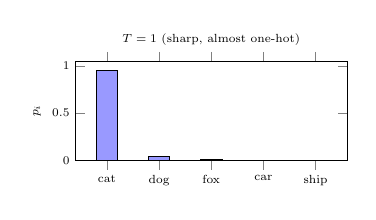
\begin{tikzpicture}[scale=0.78, every node/.style={scale=0.78}]
        \begin{axis}[
          width=6.0cm, height=3.2cm,
          ybar, bar width=10pt,
          ymin=0, ymax=1.05,
          xtick={1,2,3,4,5},
          xticklabels={cat, dog, fox, car, ship},
          x tick label style={font=\scriptsize},
          y tick label style={font=\scriptsize},
          ylabel={\scriptsize $p_i$},
          title={\scriptsize $T = 1$ (sharp, almost one-hot)},
          enlarge x limits=0.15,
        ]
          \addplot[fill=blue!40] coordinates {(1,0.95) (2,0.04) (3,0.008) (4,0.0015) (5,0.0005)};
        \end{axis}
      \end{tikzpicture}

      \vspace{0.4em}
      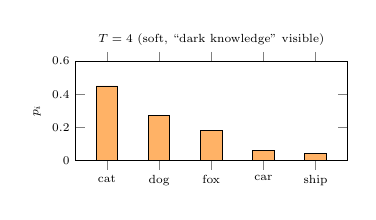
\begin{tikzpicture}[scale=0.78, every node/.style={scale=0.78}]
        \begin{axis}[
          width=6.0cm, height=3.2cm,
          ybar, bar width=10pt,
          ymin=0, ymax=0.6,
          xtick={1,2,3,4,5},
          xticklabels={cat, dog, fox, car, ship},
          x tick label style={font=\scriptsize},
          y tick label style={font=\scriptsize},
          ylabel={\scriptsize $p_i$},
          title={\scriptsize $T = 4$ (soft, ``dark knowledge'' visible)},
          enlarge x limits=0.15,
        ]
          \addplot[fill=orange!60] coordinates {(1,0.45) (2,0.27) (3,0.18) (4,0.06) (5,0.04)};
        \end{axis}
      \end{tikzpicture}

      \vspace{0.3em}
      {\scriptsize At $T=4$ the student sees: \emph{cat is much more like dog and fox than like car and ship}.}
    \end{column}
  \end{columns}
\end{frame}

\subsection{KL on Logits vs Cross-Entropy on Labels}

% -----------------------------------------------------------------------
\begin{frame}{Why KL on Logits Beats CE on Hard Labels}
  Hard labels carry only $\log_2 K$ bits per example. Teacher distributions carry the \emphdef{full predictive vector}, encoding several non-trivial signals at once.

  \vspace{0.3em}
  \begin{description}
    \item[Dark knowledge:] Relative scores of \emph{wrong} classes encode the teacher's similarity structure (cat$\sim$dog, truck$\sim$car). One-hot labels destroy this.
    \item[Dense gradient signal:] CE on a one-hot label provides a single nonzero target component; KL with a soft teacher provides gradient on every output dimension.
    \item[Implicit regularization:] Soft targets are a label-smoothing prior derived from a model that has actually seen the data, so they smooth in the right directions.
    \item[Calibrated confidence:] On ambiguous inputs the teacher hedges; the student inherits well-calibrated uncertainty instead of over-confident one-hots.
    \item[Noise robustness:] Wrong or ambiguous labels matter less because the teacher's distribution dominates the loss.
  \end{description}
\end{frame}

% -----------------------------------------------------------------------
\begin{frame}{Information per Example: Bits Argument}
  \begin{columns}[T]
    \begin{column}{0.48\textwidth}
      \textbf{One-hot label:}
      \begin{itemize}[nosep]
        \item $\log_2 K$ bits per token
        \item Vocab $K = 32{,}000 \Rightarrow \approx 15$ bits
        \item All ``other'' classes look identical (zero)
      \end{itemize}

      \vspace{0.4em}
      \textbf{Teacher distribution:}
      \begin{itemize}[nosep]
        \item Real number per class, $\sim K$ values
        \item Encodes ranking, magnitudes, similarities
        \item Bits per example bounded only by precision and entropy
      \end{itemize}

      \vspace{0.4em}
      \textbf{RL reward (for contrast):}
      \begin{itemize}[nosep]
        \item One scalar per \emph{trajectory}
        \item $\mathcal{O}(1)$ bits per episode
      \end{itemize}
    \end{column}
    \begin{column}{0.50\textwidth}
      \begin{tcolorbox}[colback=blue!5, colframe=blue!40, boxrule=0.5pt, arc=2pt, left=4pt, right=4pt, top=3pt, bottom=3pt]
      \textbf{Rule of thumb}~\cite{thinkingmachines2025distillation}:
      \begin{itemize}[nosep]
        \item RL teaches $\mathcal{O}(1)$ bits per episode
        \item Distillation teaches $\mathcal{O}(N)$ bits per episode, where $N$ is the number of tokens
        \item SFT teaches $\mathcal{O}(N \log_2 K)$ bits, but along a single sample only
      \end{itemize}
      \end{tcolorbox}

      \vspace{0.3em}
      \textbf{Consequence:} A distilled gradient step is much more informative than an RL step or an SFT step on a one-hot target. In practice this translates to many fewer optimizer steps and much smaller datasets needed to reach a given quality level.
    \end{column}
  \end{columns}
\end{frame}

% -----------------------------------------------------------------------
\begin{frame}{Dark Knowledge: A Concrete Example}
  Teacher prediction on an image of a BMW:

  \vspace{0.4em}
  \begin{center}
    \begin{tabular}{l c c}
      \toprule
      \textbf{Class} & \textbf{Teacher $p_T$} & \textbf{Hard label} \\
      \midrule
      \textcolor{blue!60!black}{car}      & $0.90$                   & $1$ \\
      truck    & $0.07$                   & $0$ \\
      bus      & $0.025$                  & $0$ \\
      garbage truck & $0.004$            & $0$ \\
      \midrule
      cat      & $3 \times 10^{-7}$       & $0$ \\
      dog      & $2 \times 10^{-7}$       & $0$ \\
      \bottomrule
    \end{tabular}
  \end{center}

  \vspace{0.4em}
  \begin{itemize}[nosep]
    \item The teacher tells the student: this looks ``a bit like a truck or bus, almost nothing like a cat''.
    \item One-hot loss treats truck and cat equivalently as ``not the answer''.
    \item Distillation loss penalizes confusing a BMW with a cat much more than confusing it with a truck, mirroring how a good model \emph{should} fail.
  \end{itemize}
\end{frame}

\subsection{Self-Distillation}

% -----------------------------------------------------------------------
\begin{frame}{Self-Distillation: Student = Teacher Architecture}
  \emphdef{Self-distillation}: distill into a model with the \emph{same} (or even smaller) architecture as the teacher. Surprisingly, this often \emph{improves} accuracy.

  \vspace{0.3em}
  \begin{description}
    \item[Born-Again Networks~\cite{furlanello2018born}:] Train net $M_0$ normally, then train $M_1$ with the same architecture using $M_0$ as teacher. Repeat. Final ensemble or $M_k$ outperforms $M_0$.
    \item[Be Your Own Teacher~\cite{zhang2019selfdistillation}:] Within a single CNN, deeper sections supervise shallower sections via auxiliary classifiers. No external teacher.
    \item[Online self-distillation:] Use an EMA of the student's own weights as a moving teacher (cf.\ BYOL, mean teacher).
  \end{description}

  \vspace{0.3em}
  \textbf{Why does it work?} Several plausible explanations:
  \begin{itemize}[nosep]
    \item Soft targets act as data-dependent label smoothing, reducing overconfidence
    \item Teacher logits encode similarity structure that hard labels destroy
    \item The teacher passes a model whose classes align with the student's inductive bias
    \item Gradient signal is denser and easier to optimize
  \end{itemize}
\end{frame}

% -----------------------------------------------------------------------
\begin{frame}{Born-Again Networks}
  \begin{center}
    \begin{tikzpicture}[
      scale=0.9, every node/.style={scale=0.9},
      net/.style={rectangle, draw, rounded corners, fill=blue!12, minimum width=1.7cm, minimum height=1.0cm, align=center, font=\small},
      label/.style={font=\scriptsize, text=gray, align=center},
      arr/.style={-{Stealth[length=5pt]}, thick},
      distill/.style={-{Stealth[length=4pt]}, thick, orange!70!black, dashed},
    ]
      \node[net] (m0) at (0, 0) {$M_0$};
      \node[net] (m1) at (2.6, 0) {$M_1$};
      \node[net] (m2) at (5.2, 0) {$M_2$};
      \node[net, fill=green!15] (mk) at (8.4, 0) {$M_k$};
      \node[font=\Large] at (6.8, 0) {$\cdots$};

      \node[label] at (0, -1.0) {hard labels\\$y$};
      \node[label] at (2.6, -1.0) {teacher $M_0$\\soft targets};
      \node[label] at (5.2, -1.0) {teacher $M_1$\\soft targets};
      \node[label] at (8.4, -1.0) {teacher $M_{k-1}$\\soft targets};

      \draw[distill] (m0) -- (m1);
      \draw[distill] (m1) -- (m2);
      \draw[distill] (m2) -- (6.4, 0);
      \draw[distill] (7.2, 0) -- (mk);

      \node[label, text=red!70!black] at (4.2, 1.4) {same architecture, fresh init each step};
      \draw[gray, dashed] (-0.7, 0.6) rectangle (9.1, 1.0);
    \end{tikzpicture}
  \end{center}

  \vspace{0.4em}
  \textbf{Empirical observation:} $M_k$ keeps improving over $M_0$ for several generations, then saturates. The trick is essentially free supervision from a model that has already digested the dataset.
\end{frame}

\subsection{On-Policy Distillation}

% -----------------------------------------------------------------------
\begin{frame}{Off-Policy vs On-Policy Distillation}
  Two ways to source the inputs the student trains on:

  \vspace{0.3em}
  \begin{description}
    \item[Off-policy (classical):] Use sequences sampled from the \emph{teacher} (or a fixed dataset). The student is trained to imitate teacher tokens given teacher prefixes.
    \item[On-policy~\cite{agarwal2024gkd,thinkingmachines2025distillation}:] Sample sequences from the \emph{student} itself, then ask the teacher to score them. The student trains on \emph{its own} mistakes.
  \end{description}

  \vspace{0.3em}
  \begin{center}
    \begin{tikzpicture}[
      scale=0.85, every node/.style={scale=0.85},
      box/.style={rectangle, draw, rounded corners, minimum width=2.2cm, minimum height=0.7cm, align=center, font=\scriptsize},
      arr/.style={-{Stealth[length=4pt]}, thick},
    ]
      % Off-policy
      \node[font=\small\bfseries] at (-3.5, 2.4) {Off-policy};
      \node[box, fill=blue!15] (T1) at (-5, 1.5) {Teacher};
      \node[box, fill=gray!15] (s1) at (-5, 0.4) {teacher rollouts};
      \node[box, fill=green!15] (S1) at (-2, 0.95) {Student};
      \draw[arr] (T1) -- (s1);
      \draw[arr] (s1) -- (S1);
      \node[font=\scriptsize, text=gray] at (-3.5, -0.4) {distribution mismatch at inference};

      % On-policy
      \node[font=\small\bfseries] at (3.5, 2.4) {On-policy};
      \node[box, fill=green!15] (S2) at (2, 1.5) {Student};
      \node[box, fill=gray!15] (s2) at (5, 1.5) {student rollouts};
      \node[box, fill=blue!15] (T2) at (5, 0.4) {Teacher};
      \node[box, fill=orange!20] (loss) at (2, 0.4) {KL loss};
      \draw[arr] (S2) -- (s2);
      \draw[arr] (s2) -- (T2);
      \draw[arr] (T2) -- (loss);
      \draw[arr] (loss) -- (S2);
      \node[font=\scriptsize, text=gray] at (3.5, -0.4) {trains on its own state distribution};
    \end{tikzpicture}
  \end{center}

  \textbf{Exposure bias:} Off-policy training never shows the student its own error states, so small mistakes at inference time compound. On-policy fixes this by definition.
\end{frame}

% -----------------------------------------------------------------------
\begin{frame}{Forward vs Reverse KL}
  \begin{columns}[T]
    \begin{column}{0.50\textwidth}
      \textbf{Forward KL} (used by SFT, off-policy KD):
      \[
        \mathrm{KL}(\pi_T \,\Vert\, \pi_\theta) = \E_{x \sim \pi_T}\!\left[\log\tfrac{\pi_T(x)}{\pi_\theta(x)}\right]
      \]
      \begin{itemize}[nosep]
        \item Samples drawn from \emph{teacher}
        \item \emphdef{Mode-covering}: penalizes any $x$ where $\pi_T > 0$ but $\pi_\theta \approx 0$
        \item Student spreads mass to cover all teacher modes, including bad ones
        \item Can be ``hacked'': $\pi_\theta$ assigns a tiny probability to garbage to keep KL low
      \end{itemize}

      \vspace{0.4em}
      \textbf{Reverse KL} (used by on-policy distillation):
      \[
        \mathrm{KL}(\pi_\theta \,\Vert\, \pi_T) = \E_{x \sim \pi_\theta}\!\left[\log\tfrac{\pi_\theta(x)}{\pi_T(x)}\right]
      \]
      \begin{itemize}[nosep]
        \item Samples drawn from \emph{student} (on-policy!)
        \item \emphdef{Mode-seeking}: forces student mass to land on teacher-approved regions
        \item Low reverse KL $\Rightarrow$ student behavior is provably teacher-like
      \end{itemize}
    \end{column}
    \begin{column}{0.46\textwidth}
      \centering
      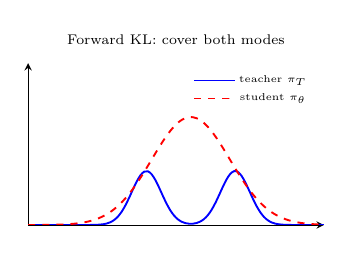
\begin{tikzpicture}[scale=0.85, every node/.style={scale=0.85}]
        \begin{axis}[
          width=6.0cm, height=4.0cm,
          xmin=-4, xmax=6, ymin=0, ymax=0.6,
          xtick=\empty, ytick=\empty,
          axis lines=left,
          title={\scriptsize Forward KL: cover both modes},
          legend style={font=\tiny, draw=none, fill=none, at={(0.98,0.98)}, anchor=north east},
        ]
          \addplot[blue, thick, smooth, domain=-4:6, samples=80] {0.5 * (0.4*exp(-(x-0)^2/0.5) + 0.4*exp(-(x-3)^2/0.5))};
          \addlegendentry{teacher $\pi_T$}
          \addplot[red, thick, smooth, dashed, domain=-4:6, samples=80] {0.4*exp(-(x-1.5)^2/3.5)};
          \addlegendentry{student $\pi_\theta$}
        \end{axis}
      \end{tikzpicture}

      \vspace{0.2em}
      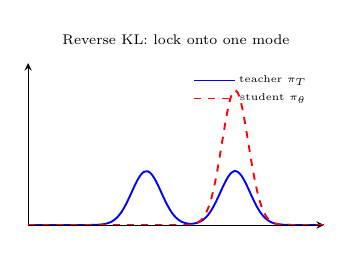
\begin{tikzpicture}[scale=0.85, every node/.style={scale=0.85}]
        \begin{axis}[
          width=6.0cm, height=4.0cm,
          xmin=-4, xmax=6, ymin=0, ymax=0.6,
          xtick=\empty, ytick=\empty,
          axis lines=left,
          title={\scriptsize Reverse KL: lock onto one mode},
          legend style={font=\tiny, draw=none, fill=none, at={(0.98,0.98)}, anchor=north east},
        ]
          \addplot[blue, thick, smooth, domain=-4:6, samples=80] {0.5 * (0.4*exp(-(x-0)^2/0.5) + 0.4*exp(-(x-3)^2/0.5))};
          \addlegendentry{teacher $\pi_T$}
          \addplot[red, thick, smooth, dashed, domain=-4:6, samples=80] {0.5*exp(-(x-3)^2/0.4)};
          \addlegendentry{student $\pi_\theta$}
        \end{axis}
      \end{tikzpicture}
    \end{column}
  \end{columns}
\end{frame}

% -----------------------------------------------------------------------
\begin{frame}{On-Policy Distillation Algorithm}
  \begin{algorithm}[H]
  \small
  \caption{On-Policy Distillation~\cite{agarwal2024gkd,thinkingmachines2025distillation}}
  \KwInput{Student $\pi_\theta$, frozen teacher $\pi_T$, prompt set $\mathcal{P}$, learning rate $\alpha$}
  \For{$k = 0$ \KwTo $K-1$}{
    Sample prompts $x \sim \mathcal{P}$\;
    \textbf{Student rollout:} generate $y = (y_1, \dots, y_N) \sim \pi_\theta(\cdot \mid x)$\;
    \textbf{Teacher scoring:} query $\log \pi_T(y_t \mid x, y_{<t})$ for every token (single forward pass)\;
    \textbf{Per-token reward:} $r_t = -\bigl(\log \pi_\theta(y_t \mid \cdot) - \log \pi_T(y_t \mid \cdot)\bigr)$ \tcp*{negative reverse KL}
    \textbf{Loss:} $\mathcal{L}(\theta) = -\E\!\left[\sum_t r_t\right]$ (with importance sampling for off-policy steps)\;
    Update $\theta \leftarrow \theta + \alpha \, \nabla_\theta(-\mathcal{L})$\;
  }
  \end{algorithm}

  \vspace{0.3em}
  \begin{itemize}[nosep]
    \item Looks like RL with REINFORCE / GRPO, but the reward is \emph{dense} and \emph{differentiable through the teacher}.
    \item No reward model, no human labels, no verifier needed: the teacher is the reward.
    \item Same data can be reused for many epochs (low memorization risk because the student keeps generating new rollouts).
  \end{itemize}
\end{frame}

% -----------------------------------------------------------------------
\begin{frame}{Why On-Policy Distillation Wins}
  \begin{description}
    \item[Dense reward:] Per-token reverse KL gives a learning signal on \emph{every} token, not just the final answer. $\mathcal{O}(N)$ bits per episode vs RL's $\mathcal{O}(1)$.
    \item[On-policy:] The student trains on the exact state distribution it will encounter at inference time, eliminating exposure bias and teacher/student mismatch.
    \item[Mode-seeking:] Reverse KL is ``unhackable''. Low KL implies the student's actual rollouts are teacher-approved, not just that they have nonzero probability under the teacher.
    \item[Differentiable critic:] The teacher acts as a frozen, perfect dense critic; no need to train a reward model.
    \item[Data efficiency:] Multi-epoch reuse is safe because each epoch generates fresh student rollouts, unlike SFT which can memorize.
  \end{description}

  \vspace{0.3em}
  \begin{tcolorbox}[colback=green!5, colframe=green!50!black, boxrule=0.5pt, arc=2pt, left=4pt, right=4pt, top=3pt, bottom=3pt]
  \textbf{Slogan}~\cite{thinkingmachines2025distillation}: ``On-policy training, off-policy reward signal''.
  \end{tcolorbox}
\end{frame}

% -----------------------------------------------------------------------
\begin{frame}{Empirical Results: Math Reasoning}
  Distilling Qwen3-32B into Qwen3-8B on AIME'24~\cite{thinkingmachines2025distillation}:

  \vspace{0.4em}
  \begin{center}
  \renewcommand{\arraystretch}{1.15}
  \begin{tabular}{l c c}
    \toprule
    \textbf{Method} & \textbf{AIME'24} & \textbf{GPU-hours} \\
    \midrule
    SFT on 400k teacher traces            & $60.0\%$  & (baseline)        \\
    RL from scratch (verifier)            & $67.6\%$  & $17{,}920$        \\
    \rowcolor{green!10}
    On-policy distillation                & $\mathbf{74.4\%}$ & $\mathbf{1{,}800}$ \\
    \bottomrule
  \end{tabular}
  \end{center}

  \vspace{0.3em}
  \begin{itemize}[nosep]
    \item On-policy distillation \emph{beats} RL while using $\sim$10$\times$ less compute.
    \item Including the SFT data amortization, end-to-end savings are $50$--$100\times$ vs running RL alone.
    \item Reaches teacher performance in $7$--$10\times$ fewer gradient steps than RL, thanks to dense per-token rewards.
  \end{itemize}
\end{frame}

% -----------------------------------------------------------------------
\begin{frame}{Recovering Capabilities Lost to Mid-Training}
  \textbf{Setting:} Take a strong post-trained model (Qwen3-8B post-trained), then mid-train it on internal company documents to inject domain knowledge. Instruction-following collapses.

  \vspace{0.3em}
  \begin{center}
  \renewcommand{\arraystretch}{1.15}
  \begin{tabular}{l c c}
    \toprule
    \textbf{Stage} & \textbf{Knowledge} & \textbf{Instruction following} \\
    \midrule
    Post-trained baseline                       & $\sim 18\%$ & $\sim 85\%$ \\
    + mid-train on internal docs                & $43\%$      & $45\%$      \\
    \rowcolor{green!10}
    + on-policy distillation from baseline      & $41\%$      & $\mathbf{83\%}$ \\
    \bottomrule
  \end{tabular}
  \end{center}

  \vspace{0.3em}
  \begin{itemize}[nosep]
    \item The teacher is the model's own pre-mid-training self.
    \item The student keeps the new domain knowledge and recovers almost all of the lost instruction-following ability.
    \item On-policy distillation acts as a targeted ``unforgetting'' mechanism: the LM itself is the reward model.
  \end{itemize}
\end{frame}

% -----------------------------------------------------------------------
\begin{frame}{Summary}
  \begin{description}
    \item[Distillation:] Train a student to match a teacher's full distribution. Compresses models, transfers skills, and recovers capabilities.
    \item[Why logits not labels?] Soft targets carry dark knowledge, give dense gradients, smooth labels in data-aware ways, and preserve calibration.
    \item[Self-distillation:] Even when teacher = student architecture, soft-target supervision improves accuracy (born-again networks, be-your-own-teacher).
    \item[On-policy distillation:] Sample from the student, score with a frozen teacher, minimize per-token reverse KL. Combines RL's on-policy state distribution with SFT's dense supervision.
    \item[In practice:] Fewer GPU-hours than RL, no reward model, robust to multi-epoch reuse, and applicable to compression, reasoning transfer, and capability recovery.
  \end{description}
\end{frame}
